
\documentclass{beamer}

\usetheme{Copenhagen}

\title{Matrix Project}
\subtitle{EE1390- Intro to AI and ML}
\usepackage{graphicx}
\graphicspath{{./images/}}

\author[]{Md.Sadiq - EE18BTECH11051 
\\
S.Abdur Rahman Nawaz - EE18BTECH11052}


\date{14-02-2013}

\subject{JEE questions solving using python}

\AtBeginSubsection[]
{
  \begin{frame}<beamer>{Outline}
    \tableofcontents[currentsection,currentsubsection]
  \end{frame}
}

\begin{document}

\begin{frame}
  \titlepage
\end{frame}

\begin{frame}{Outline}
  \tableofcontents
\end{frame}

\section{Question}

\begin{frame}{JEE Question}
 
 
   Q. Find the Equation of the circle, which is mirror image of the circle\\
$\mathbf{x}^\intercal \mathbf{x}$ - $\begin{pmatrix} 2\ 0 \end{pmatrix}\mathbf{x}$ = 0
\\and the line\\
$\begin{pmatrix} 1\ 1 \end{pmatrix}\mathbf{x}$ = 3
\end{frame}

\section{Solution}
\begin{frame}{Solution}
THE BASIC IDEA OF THIS APPROACH IS TO FIND THE CENTRE OF THE CIRCLE
 FROM THE GIVEN EQUATION, AND FINDING IT'S REFLECTION IN THE LINE
 AS THE REFLECTION OF A CIRCLE IS A CIRCLE WITH EQUAL RADIUS, WE KNOW
 THAT THE ONLY THING TO FIND IS THE REFLECTION OF CENTRE AND PLOT A
 CIRCLE OF EQUAL RADIUS AROUND IT. THIS IS THE REFLECTED CIRCLE.
\end{frame}

\begin{frame}{Solution}
As the equation of the circle is
$\mathbf{x}^\intercal \mathbf{x}$ - $\begin{pmatrix} 2\ 0 \end{pmatrix}\mathbf{x}$ = 0
,its centre is $1/2*\begin{pmatrix} 2\ 0 \end{pmatrix}$ = $\begin{pmatrix} 1\ 0 \end{pmatrix}$
Equation of given line is $\mathbf{n_{1}}^\intercal \mathbf{x} = p_{1}$,
Here n_{1} = $\begin{pmatrix} 1\ 1 \end{pmatrix}$  and\  $p_{1} = 3$
And let the equation of line passing through centre of circle and perpendicular to the given line be
 $\mathbf{n_{2}}^\intercal \mathbf{x} = p_{2}$

Now that can be written as $\begin{pmatrix}\mathbf{n_{1}}^\intercal \\ \mathbf{n_{2}}^\intercal \end{pmatrix}$ $\mathbf{x} = \begin{pmatrix} p{1}\\ p{2} \end{pmatrix}\ $
or $\mathbf{N}^\intercal\mathbf{x} = \mathbf{p}$ 
 and $\mathbf{x}=(\mathbf{N}^\intercal)^{-1}\mathbf{p}$ which is the point of intersection of the given line and the normal to the circle which is also normal to the given line.

\end{frame}

\begin{frame}{Solution}
Now, $ 2*\mathbf{x} - \mathbf{C} $ Where C is the centre of the given circle would give us the reflection of the centre of the given circle.

And now since we know that Radius of the Circle won't change in reflection.
Circle can be easily plotted by using the centre and radius
\end{frame}

\section{Graphical representation}

\begin{frame}{Graphical representation}
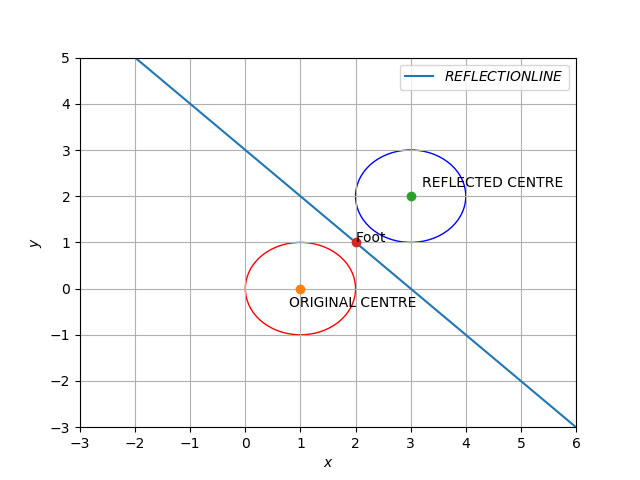
\includegraphics[scale =0.6]{Figure_1.png}
\end{frame}

\begin{frame}{Final Slide}
\begin{center}
    THANK YOU
\end{center}
    
\end{frame}
    

\end{document}


